\documentclass{ximera}

%\usepackage{todonotes}

\newcommand{\todo}{}

\usepackage{esint} % for \oiint
\ifxake%%https://math.meta.stackexchange.com/questions/9973/how-do-you-render-a-closed-surface-double-integral
\renewcommand{\oiint}{{\large\bigcirc}\kern-1.56em\iint}
\fi


\graphicspath{
  {./}
  {ximeraTutorial/}
  {basicPhilosophy/}
  {functionsOfSeveralVariables/}
  {normalVectors/}
  {lagrangeMultipliers/}
  {vectorFields/}
  {greensTheorem/}
  {shapeOfThingsToCome/}
  {dotProducts/}
  {partialDerivativesAndTheGradientVector/}
  {../productAndQuotientRules/exercises/}
  {../normalVectors/exercisesParametricPlots/}
  {../continuityOfFunctionsOfSeveralVariables/exercises/}
  {../partialDerivativesAndTheGradientVector/exercises/}
  {../directionalDerivativeAndChainRule/exercises/}
  {../commonCoordinates/exercisesCylindricalCoordinates/}
  {../commonCoordinates/exercisesSphericalCoordinates/}
  {../greensTheorem/exercisesCurlAndLineIntegrals/}
  {../greensTheorem/exercisesDivergenceAndLineIntegrals/}
  {../shapeOfThingsToCome/exercisesDivergenceTheorem/}
  {../greensTheorem/}
  {../shapeOfThingsToCome/}
  {../separableDifferentialEquations/exercises/}
  {vectorFields/}
}

\newcommand{\mooculus}{\textsf{\textbf{MOOC}\textnormal{\textsf{ULUS}}}}

\usepackage{tkz-euclide}
\usepackage{tikz}
\usepackage{tikz-cd}
\usetikzlibrary{arrows}
\tikzset{>=stealth,commutative diagrams/.cd,
  arrow style=tikz,diagrams={>=stealth}} %% cool arrow head
\tikzset{shorten <>/.style={ shorten >=#1, shorten <=#1 } } %% allows shorter vectors

\usetikzlibrary{backgrounds} %% for boxes around graphs
\usetikzlibrary{shapes,positioning}  %% Clouds and stars
\usetikzlibrary{matrix} %% for matrix
\usepgfplotslibrary{polar} %% for polar plots
\usepgfplotslibrary{fillbetween} %% to shade area between curves in TikZ
%\usetkzobj{all}
\usepackage[makeroom]{cancel} %% for strike outs
%\usepackage{mathtools} %% for pretty underbrace % Breaks Ximera
%\usepackage{multicol}
\usepackage{pgffor} %% required for integral for loops



%% http://tex.stackexchange.com/questions/66490/drawing-a-tikz-arc-specifying-the-center
%% Draws beach ball
\tikzset{pics/carc/.style args={#1:#2:#3}{code={\draw[pic actions] (#1:#3) arc(#1:#2:#3);}}}



\usepackage{array}
\setlength{\extrarowheight}{+.1cm}
\newdimen\digitwidth
\settowidth\digitwidth{9}
\def\divrule#1#2{
\noalign{\moveright#1\digitwidth
\vbox{\hrule width#2\digitwidth}}}




% \newcommand{\RR}{\mathbb R}
% \newcommand{\R}{\mathbb R}
% \newcommand{\N}{\mathbb N}
% \newcommand{\Z}{\mathbb Z}

\newcommand{\sagemath}{\textsf{SageMath}}


%\renewcommand{\d}{\,d\!}
%\renewcommand{\d}{\mathop{}\!d}
%\newcommand{\dd}[2][]{\frac{\d #1}{\d #2}}
%\newcommand{\pp}[2][]{\frac{\partial #1}{\partial #2}}
% \renewcommand{\l}{\ell}
%\newcommand{\ddx}{\frac{d}{\d x}}

% \newcommand{\zeroOverZero}{\ensuremath{\boldsymbol{\tfrac{0}{0}}}}
%\newcommand{\inftyOverInfty}{\ensuremath{\boldsymbol{\tfrac{\infty}{\infty}}}}
%\newcommand{\zeroOverInfty}{\ensuremath{\boldsymbol{\tfrac{0}{\infty}}}}
%\newcommand{\zeroTimesInfty}{\ensuremath{\small\boldsymbol{0\cdot \infty}}}
%\newcommand{\inftyMinusInfty}{\ensuremath{\small\boldsymbol{\infty - \infty}}}
%\newcommand{\oneToInfty}{\ensuremath{\boldsymbol{1^\infty}}}
%\newcommand{\zeroToZero}{\ensuremath{\boldsymbol{0^0}}}
%\newcommand{\inftyToZero}{\ensuremath{\boldsymbol{\infty^0}}}



% \newcommand{\numOverZero}{\ensuremath{\boldsymbol{\tfrac{\#}{0}}}}
% \newcommand{\dfn}{\textbf}
% \newcommand{\unit}{\,\mathrm}
% \newcommand{\unit}{\mathop{}\!\mathrm}
% \newcommand{\eval}[1]{\bigg[ #1 \bigg]}
% \newcommand{\seq}[1]{\left( #1 \right)}
% \renewcommand{\epsilon}{\varepsilon}
% \renewcommand{\phi}{\varphi}


% \renewcommand{\iff}{\Leftrightarrow}

% \DeclareMathOperator{\arccot}{arccot}
% \DeclareMathOperator{\arcsec}{arcsec}
% \DeclareMathOperator{\arccsc}{arccsc}
% \DeclareMathOperator{\si}{Si}
% \DeclareMathOperator{\scal}{scal}
% \DeclareMathOperator{\sign}{sign}


%% \newcommand{\tightoverset}[2]{% for arrow vec
%%   \mathop{#2}\limits^{\vbox to -.5ex{\kern-0.75ex\hbox{$#1$}\vss}}}
% \newcommand{\arrowvec}[1]{{\overset{\rightharpoonup}{#1}}}
% \renewcommand{\vec}[1]{\arrowvec{\mathbf{#1}}}
% \renewcommand{\vec}[1]{{\overset{\boldsymbol{\rightharpoonup}}{\mathbf{#1}}}}

% \newcommand{\point}[1]{\left(#1\right)} %this allows \vector{ to be changed to \vector{ with a quick find and replace
% \newcommand{\pt}[1]{\mathbf{#1}} %this allows \vec{ to be changed to \vec{ with a quick find and replace
% \newcommand{\Lim}[2]{\lim_{\point{#1} \to \point{#2}}} %Bart, I changed this to point since I want to use it.  It runs through both of the exercise and exerciseE files in limits section, which is why it was in each document to start with.

% \DeclareMathOperator{\proj}{\mathbf{proj}}
% \newcommand{\veci}{{\boldsymbol{\hat{\imath}}}}
% \newcommand{\vecj}{{\boldsymbol{\hat{\jmath}}}}
% \newcommand{\veck}{{\boldsymbol{\hat{k}}}}
% \newcommand{\vecl}{\vec{\boldsymbol{\l}}}
% \newcommand{\uvec}[1]{\mathbf{\hat{#1}}}
% \newcommand{\utan}{\mathbf{\hat{t}}}
% \newcommand{\unormal}{\mathbf{\hat{n}}}
% \newcommand{\ubinormal}{\mathbf{\hat{b}}}

% \newcommand{\dotp}{\bullet}
% \newcommand{\cross}{\boldsymbol\times}
% \newcommand{\grad}{\boldsymbol\nabla}
% \newcommand{\divergence}{\grad\dotp}
% \newcommand{\curl}{\grad\cross}
%\DeclareMathOperator{\divergence}{divergence}
%\DeclareMathOperator{\curl}[1]{\grad\cross #1}
% \newcommand{\lto}{\mathop{\longrightarrow\,}\limits}

% \renewcommand{\bar}{\overline}

\colorlet{textColor}{black}
\colorlet{background}{white}
\colorlet{penColor}{blue!50!black} % Color of a curve in a plot
\colorlet{penColor2}{red!50!black}% Color of a curve in a plot
\colorlet{penColor3}{red!50!blue} % Color of a curve in a plot
\colorlet{penColor4}{green!50!black} % Color of a curve in a plot
\colorlet{penColor5}{orange!80!black} % Color of a curve in a plot
\colorlet{penColor6}{yellow!70!black} % Color of a curve in a plot
\colorlet{fill1}{penColor!20} % Color of fill in a plot
\colorlet{fill2}{penColor2!20} % Color of fill in a plot
\colorlet{fillp}{fill1} % Color of positive area
\colorlet{filln}{penColor2!20} % Color of negative area
\colorlet{fill3}{penColor3!20} % Fill
\colorlet{fill4}{penColor4!20} % Fill
\colorlet{fill5}{penColor5!20} % Fill
\colorlet{gridColor}{gray!50} % Color of grid in a plot

\newcommand{\surfaceColor}{violet}
\newcommand{\surfaceColorTwo}{redyellow}
\newcommand{\sliceColor}{greenyellow}




\pgfmathdeclarefunction{gauss}{2}{% gives gaussian
  \pgfmathparse{1/(#2*sqrt(2*pi))*exp(-((x-#1)^2)/(2*#2^2))}%
}


%%%%%%%%%%%%%
%% Vectors
%%%%%%%%%%%%%

%% Simple horiz vectors
\renewcommand{\vector}[1]{\left\langle #1\right\rangle}


%% %% Complex Horiz Vectors with angle brackets
%% \makeatletter
%% \renewcommand{\vector}[2][ , ]{\left\langle%
%%   \def\nextitem{\def\nextitem{#1}}%
%%   \@for \el:=#2\do{\nextitem\el}\right\rangle%
%% }
%% \makeatother

%% %% Vertical Vectors
%% \def\vector#1{\begin{bmatrix}\vecListA#1,,\end{bmatrix}}
%% \def\vecListA#1,{\if,#1,\else #1\cr \expandafter \vecListA \fi}

%%%%%%%%%%%%%
%% End of vectors
%%%%%%%%%%%%%

%\newcommand{\fullwidth}{}
%\newcommand{\normalwidth}{}



%% makes a snazzy t-chart for evaluating functions
%\newenvironment{tchart}{\rowcolors{2}{}{background!90!textColor}\array}{\endarray}

%%This is to help with formatting on future title pages.
\newenvironment{sectionOutcomes}{}{}



%% Flowchart stuff
%\tikzstyle{startstop} = [rectangle, rounded corners, minimum width=3cm, minimum height=1cm,text centered, draw=black]
%\tikzstyle{question} = [rectangle, minimum width=3cm, minimum height=1cm, text centered, draw=black]
%\tikzstyle{decision} = [trapezium, trapezium left angle=70, trapezium right angle=110, minimum width=3cm, minimum height=1cm, text centered, draw=black]
%\tikzstyle{question} = [rectangle, rounded corners, minimum width=3cm, minimum height=1cm,text centered, draw=black]
%\tikzstyle{process} = [rectangle, minimum width=3cm, minimum height=1cm, text centered, draw=black]
%\tikzstyle{decision} = [trapezium, trapezium left angle=70, trapezium right angle=110, minimum width=3cm, minimum height=1cm, text centered, draw=black]


\title{Transform}

\begin{document}

\begin{abstract}
graphs
\end{abstract}
\maketitle



When two sine functions have the same period, then their graphs (or waveforms) have the same distance between the hills and valleys.   The graphs of the two sine functions could be in synch, which means the tops of the hills and bottoms of valleys occur at the exact same angle.  In this case, we say the waveforms are \textbf{in phase}.


If one of the waveforms experiences a horizontal shift, then we say that the waveforms are \textbf{out of phase}.

If the shift makes the hills of one waveform align perfectly with the valleys of the other waveform, then we say that the two waveforms are \textbf{completely out of phase}.




\begin{example}  Sine



Compare $s(\theta) = 2 \sin\left(\theta - \frac{\pi}{4}\right) + 2$ to the basic sine curve.\\





\begin{image}
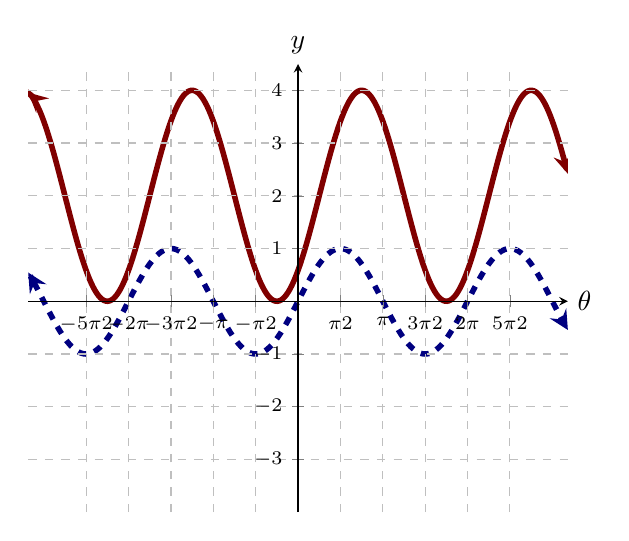
\begin{tikzpicture}
  \begin{axis}[
            domain=-10:10, ymax=4.5, xmax=10, ymin=-4, xmin=-10,
            axis lines =center, xlabel={$\theta$}, ylabel=$y$, grid = major, grid style={dashed},
            ytick={-3,-2,-1,1,2,3,4},
            xtick={-7.85, -6.28, -4.71, -3.14, -1.57, 0, 1.57, 3.142, 4.71, 6.28, 7.85},
            xticklabels={$-\tfrac{5\pi}{2}$,$-2\pi$,$-\tfrac{3\pi}{2}$,$-\pi$, $-\tfrac{\pi}{2}$, $0$, $\tfrac{\pi}{2}$, $\pi$, $\tfrac{3\pi}{2}$, $2\pi$, $\tfrac{5\pi}{2}$},
            yticklabels={$-3$,$-2$,$-1$,$1$,$2$,$3$,$4$}, 
            ticklabel style={font=\scriptsize},
            every axis y label/.style={at=(current axis.above origin),anchor=south},
            every axis x label/.style={at=(current axis.right of origin),anchor=west},
            axis on top
          ]
          

            \addplot [line width=2, penColor, dashed,samples=300,domain=(-10:10),<->] {sin(deg(x)};
            \addplot [line width=2, penColor2, smooth,samples=300,domain=(-10:10),<->] {2*sin(deg(x-0.785398))+2};



  \end{axis}
\end{tikzpicture}
\end{image}


Since $\theta$ is multiplied by $1$, the period is still $2\pi$.

These two sine waveforms are slightly out of phase.


\end{example}



\begin{definition} \textbf{\textcolor{green!50!black}{Period}} \\

The \textbf{period} of a periodic function is the (domain)length of the repeating pattern.


For sine or cosine waveforms, this is distance from one peak to the next.

\end{definition}

\begin{definition} \textbf{\textcolor{green!50!black}{Frequency}} \\

The \textbf{frequency} is the reciprocal of period.

\end{definition}














\begin{example}  Period

What is the period of the function in the previous example?



\begin{explanation}

$s(\theta) = 2 \sin\left(\theta - \frac{\pi}{4}\right) + 2$ \\


The period is the distance between cooresponding points in the waveform.  This can be found by setting the inside equal to $0$ and $2\pi$.

\begin{align*}
 0 & = \theta - \frac{\pi}{4} \\
 \frac{\pi}{4} & = \theta 
 \end{align*}

\begin{align*}
 2 \pi & = \theta - \frac{\pi}{4} \\
 \frac{9\pi}{4} & = \theta 
 \end{align*}

\[
\frac{9\pi}{4} - \frac{\pi}{4} = \frac{8\pi}{4} = 2 \pi
\]


\end{explanation}

The period is $2\pi radians$. \\

The frequency is $\frac{1}{2\pi} \tfrac{1}{radians}$. \\

\end{example}






Two waveforms of the same frequency are in phase, if their maximum and minimum magnitudes align perfectly.

If one of these waveforms is shifted by half a period, then the waveforms are said to be \textbf{out of phase}. In this case, the sum of the two waveforms can be $0$.



\[
\sin(\theta) + \sin(\theta + \pi) = 0
\]




\begin{center}
\desmos{fwuxnrac77}{400}{300}
\end{center}









\begin{definition} \textbf{\textcolor{green!50!black}{Phase Shift}}

The \textbf{phase shift} is the horizontal shift.

\end{definition}




\begin{example} Phase Shift \\


What is the phase shift for $T(\theta) = 3 \sin\left( \frac{\theta}{2}+3 \right)-2$ ?


\begin{explanation}

To find the phase shift or horizontal shift, we need to locate the beginning of the waveform.


\begin{align*}
\frac{\theta}{2}+3 &= 0 \\
\frac{\theta}{2}   &= -3 \\
\theta             &=  -6
\end{align*}
The phase shift is $-6$.  We can see this in the graph.  The beginning of the waveform has moved left to $\theta=-6$.




\begin{image}
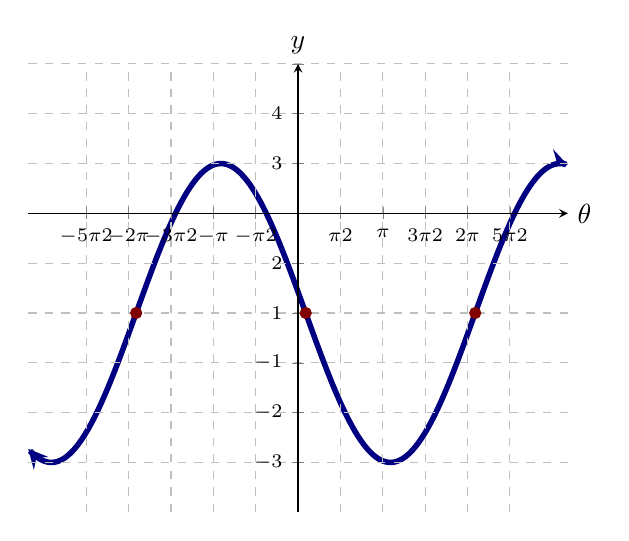
\begin{tikzpicture}
  \begin{axis}[
            domain=-10:10, ymax=3, xmax=10, ymin=-6, xmin=-10,
            axis lines =center, xlabel={$\theta$}, ylabel=$y$, grid = major, grid style={dashed},
            ytick={-5,-4,-3,-2,-1,1,2,3,4},
            xtick={-7.85, -6.28, -4.71, -3.14, -1.57, 0, 1.57, 3.142, 4.71, 6.28, 7.85},
            xticklabels={$-\tfrac{5\pi}{2}$,$-2\pi$,$-\tfrac{3\pi}{2}$,$-\pi$, $-\tfrac{\pi}{2}$, $0$, $\tfrac{\pi}{2}$, $\pi$, $\tfrac{3\pi}{2}$, $2\pi$, $\tfrac{5\pi}{2}$},
            yticklabels={$-3$,$-2$,$-1$,$1$,$2$,$3$,$4$}, 
            ticklabel style={font=\scriptsize},
            every axis y label/.style={at=(current axis.above origin),anchor=south},
            every axis x label/.style={at=(current axis.right of origin),anchor=west},
            axis on top
          ]
          

            %\addplot [line width=2, penColor, dashed,samples=300,domain=(-10:10),<->] {sin(deg(x)};
            \addplot [line width=2, penColor, smooth,samples=300,domain=(-10:10),<->] {3*sin(deg(x/2 + 3))-2};

            \addplot[color=penColor2,fill=penColor2,only marks,mark=*] coordinates{(-6,-2)};
            \addplot[color=penColor2,fill=penColor2,only marks,mark=*] coordinates{(0.283,-2)};
            \addplot[color=penColor2,fill=penColor2,only marks,mark=*] coordinates{(6.566,-2)};



  \end{axis}
\end{tikzpicture}
\end{image}






\end{explanation}



\end{example}












\begin{center}
\textbf{\textcolor{green!50!black}{ooooo-=-=-=-ooOoo-=-=-=-ooooo}} \\

more examples can be found by following this link\\ \link[More Examples of Trigonometric Graphs]{https://ximera.osu.edu/csccmathematics/precalculus2/precalculus2/trigonometricGraphs/examples/exampleList}

\end{center}





\end{document}

